\documentclass{beamer}
\usepackage{geometry}
\usepackage[english]{babel}
\usepackage[utf8]{inputenc}
\usepackage{amsmath}
\usepackage{amsfonts}
\usepackage{amssymb}
\usepackage{tikz}
\usetikzlibrary{quotes, angles}
\usepackage{graphicx}

%\usepackage{pgfplots}
%\pgfplotsset{width=10cm,compat=1.9}
%\usepackage{pgfplotstable}

\setlength{\headheight}{26pt}%doesn't seem to fix warning

\usepackage{fancyhdr}
\pagestyle{fancy}
\fancyhf{}

%\rhead{\small{13 November 2018}}
\lhead{\small{BECA / Dr. Huson / Geometry Unit 4}}

\renewcommand{\headrulewidth}{0pt}

\title{Mathematics Class Slides}
\subtitle{Bronx Early College Academy}
\author{Chris Huson}
\date{26 November 2018} % 4 December revision, add HL

\begin{document}
\frame{\titlepage}
\section[Outline]{}
\frame{\tableofcontents}


\section{4.1 Project: Triangle congruence project, Monday 26 November}
  \frame
  {
    \frametitle{Construction project: Triangle congruence}
    \framesubtitle{CCSS: HSG.CO.C.9 Prove geometric theorems \hspace{\stretch{1}} \alert{4.1}}

    \begin{block}{Four pages of $\triangle$ duplication for your binder}
    \begin{enumerate}
        \item Side-side-side (SSS $\triangle \cong$)\\
        $\triangle ABC \cong \triangle A'B'C'$ iff $\overline{AB} \cong \overline{A'B'}, \overline{BC} \cong \overline{B'C'}, \text{ and } \overline{AC} \cong \overline{A'C'}$
        \item Side-angle-side (SAS)
        \item Angle-side-angle (ASA)
        \item Side-side-angle (SSA), false, ``ambiguous case"
    \end{enumerate}
    \end{block}
    Function notation: $A \rightarrow A'$ is pronounced ``A gets mapped to A prime," or ``A corresponds to A prime."

    }

  \section{SSS Triangle congruence. Monday 26 November}
    \frame
    {
      \frametitle{SSS Triangle congruence (``side-side-side")}

      Given $\triangle ABC$, duplicate $\triangle ABC$ by duplicating each side.
      \begin{enumerate}
        \item Construct $\overrightarrow{A'}$.
        \item Circle $A'$ with radius $AB$. Intersection $B'$.
        \item Circle $A'$ with radius $AC$.
        \item Circle $B'$ with radius $BC$. Intersection $C'$.
        \item $\triangle ABC \cong \triangle A'B'C'$ by the SSS $\triangle \cong$ Postulate.
      \end{enumerate}
      \begin{tikzpicture}[scale=0.6]
        \draw [thick] (0,0)--(5.5,0)--(3,4)--cycle;
        \draw [fill] (0,0) circle [radius=0.05] node[left]{$A$};
        \draw [fill] (5.5,0) circle [radius=0.05] node[right]{$B$};
        \draw [fill] (3,4) circle [radius=0.05] node[above]{$C$};
        \draw[thick,red] ([shift=(-10:5.5)]0,0) arc (-10:10:5.5);
        \draw[thick,red] ([shift=(45:5)]0,0) arc (45:65:5);
        \draw[thick,red] ([shift=(110:4.72)]5.5,0) arc (110:130:5.5);
      \end{tikzpicture}
      \begin{tikzpicture}[scale=0.6]
        \draw [thick] (0,0)--(5.5,0)--(3,4)--cycle;
        \draw [->, thick] (0,0)--(7.5,0);
        \draw [fill] (0,0) circle [radius=0.05] node[left]{$A'$};
        \draw [fill] (5.5,0) circle [radius=0.05] node[below right]{$B'$};
        \draw [fill] (3,4) circle [radius=0.05] node[above]{$C'$};
        \draw[thick,red] ([shift=(-10:5.5)]0,0) arc (-10:10:5.5);
        \draw[thick,red] ([shift=(45:5)]0,0) arc (45:65:5);
        \draw[thick,red] ([shift=(110:4.72)]5.5,0) arc (110:130:5.5);
      \end{tikzpicture}
    }

  \section{SAS Triangle congruence. Tuesday 27 November}
    \frame
    {
      \frametitle{SAS Triangle congruence (``side-angle-side")}
      \begin{enumerate}
        \item Given $\triangle ABC$, construct a duplicate $\triangle A'B'C'$
        \item Duplicate side $\overline{AB}$, duplicate $\angle A$, duplicate side $\overline{AC}$
        \item Angle must be the \emph{included} angle, between the two sides
        \item $\triangle ABC \cong \triangle A'B'C'$ iff $\overline{AB} \cong \overline{A'B'}, \angle A \cong \angle A', \text{ \& } \overline{AC} \cong \overline{A'C'}$
      \end{enumerate}
      \begin{tikzpicture}[scale=0.6]
        \draw [thick] (0,0)--(5.5,0)--(3,4)--cycle;
        \draw [fill] (0,0) circle [radius=0.05] node[left]{$A$};
        \draw [fill] (5.5,0) circle [radius=0.05] node[right]{$B$};
        \draw [fill] (3,4) circle [radius=0.05] node[above]{$C$};
        \draw[thick, red] ([shift=(-10:5.5)]0,0) arc (-10:10:5.5);
        \draw[thick, dashed,red] ([shift=(-5:3)]0,0) arc (-5:60:3);
        \draw[thick, dashed,red] ([shift=(110:2.7)]3,0) arc (110:130:2.7);
        \draw[thick, dotted,red] ([shift=(45:5)]0,0) arc (45:65:5);
      \end{tikzpicture}
      \begin{tikzpicture}[scale=0.6]
        \draw [thick] (5.5,0)--(3,4);
        \draw [->, thick] (0,0)--(7.5,0);
        \draw [->, thick] (0,0)--(3,4)--(3.9,5.2);
        \draw [fill] (0,0) circle [radius=0.05] node[left]{$A'$};
        \draw [fill] (5.5,0) circle [radius=0.05] node[below right]{$B'$};
        \draw [fill] (3,4) circle [radius=0.05] node[right]{$C'$};
        \draw[thick, red] ([shift=(-10:5.5)]0,0) arc (-10:10:5.5);
        \draw[thick, dashed,red] ([shift=(-5:3)]0,0) arc (-5:60:3);
        \draw[thick, dashed,red] ([shift=(110:2.7)]3,0) arc (110:130:2.7);
        \draw[thick, dotted,red] ([shift=(45:5)]0,0) arc (45:65:5);
      \end{tikzpicture}
    }

  \section{ASA Triangle congruence. Wednesday 28 November}
    \frame
    {
      \frametitle{ASA Triangle congruence (``angle-side-angle")}
      \begin{enumerate}
        \item Given $\triangle ABC$, construct a duplicate $\triangle A'B'C'$
        \item Duplicate $\angle A$, duplicate side $\overline{AB}$, duplicate $\angle B$
        \item One side and \emph{any} two angles ("AAS" is ok)
        \item $\triangle ABC \cong \triangle A'B'C'$ iff $\angle A \cong \angle A', \overline{AB} \cong \overline{A'B'}, \text{ \& } \angle B \cong \angle B'$
      \end{enumerate}
      \begin{tikzpicture}[scale=0.6]
        \draw [thick] (0,0)--(5.5,0)--(3,4)--cycle;
        \draw [fill] (0,0) circle [radius=0.05] node[left]{$A$};
        \draw [fill] (5.5,0) circle [radius=0.05] node[right]{$B$};
        \draw [fill] (3,4) circle [radius=0.05] node[above]{$C$};
        \draw[thick, dashed,red] ([shift=(-10:5.5)]0,0) arc (-10:10:5.5);
        \draw[thick, red] ([shift=(-5:2)]0,0) arc (-5:60:2);
        \draw[thick, red] ([shift=(100:1.8)]2,0) arc (100:135:1.8);
        \draw[thick, dotted, red] ([shift=(110:2.5)]5.5,0) arc (110:185:2.5);
        \draw[thick, dotted, red] ([shift=(45:2.5)]3,0) arc (45:75:2.3);
      \end{tikzpicture}
      \begin{tikzpicture}[scale=0.6]
        \draw [->, thick] (5.5,0)--(3,4)--(2.5,4.8);
        \draw [->, thick] (0,0)--(7.5,0);
        \draw [->, thick] (0,0)--(3,4)--(3.9,5.2);
        \draw [fill] (0,0) circle [radius=0.05] node[left]{$A'$};
        \draw [fill] (5.5,0) circle [radius=0.05] node[below right]{$B'$};
        \draw [fill] (3,4) circle [radius=0.05] node[right]{$C'$};
        \draw[thick, dashed,red] ([shift=(-10:5.5)]0,0) arc (-10:10:5.5);
        \draw[thick, red] ([shift=(-5:2)]0,0) arc (-5:60:2);
        \draw[thick, red] ([shift=(100:1.8)]2,0) arc (100:135:1.8);
        \draw[thick, dotted, red] ([shift=(110:2.5)]5.5,0) arc (110:185:2.5);
        \draw[thick, dotted, red] ([shift=(45:2.5)]3,0) arc (45:75:2.3);
      \end{tikzpicture}
    }

  \section{SSA Triangle congruence. Thursday 29 November}
    \frame
    {
      \frametitle{SSA \emph{false} congruence (ASS or ``jack ass theorem")}
      \begin{enumerate}
        \item Given $\triangle ABC$, two $\triangle$s may have two pairs of congruent sides and a \emph{non-included} congruent angle.
        \item This is called the ``ambiguous case"
        %\item $\triangle ABC \cong \triangle A'B'C'$ iff $\overline{AB} \cong \overline{A'B'}, \angle A \cong \angle A', \text{ \& } \overline{AC} \cong \overline{A'C'}$
      \end{enumerate}
      \begin{tikzpicture}[scale=0.6]
        \draw [thick] (0,0)--(5.5,0)--(4,3.5)--cycle;
        \draw [fill] (0,0) circle [radius=0.05] node[left]{$A$};
        \draw [fill] (5.5,0) circle [radius=0.05] node[right]{$B$};
        \draw [fill] (4,3.5) circle [radius=0.05] node[above]{$C$};
        \draw[thick, dashed, red] ([shift=(-8:5.5)]0,0) arc (-8:8:5.5);
        %\draw[thick, red] ([shift=(0:0.75)]0,0) arc (0:37:0.75);
        \draw[thick, red] ([shift=(-5:2)]0,0) arc (-5:60:2);
        \draw[thick, red] ([shift=(100:1.4)]2,0) arc (100:135:1.4);
        \draw[thick, dotted, red] ([shift=(110:3.81)]5.5,0) arc (110:160:3.81);
      \end{tikzpicture}
      \begin{tikzpicture}[scale=0.6]
        \draw [dashed, thick] (5.5,0)--(4,3.5);
        \draw [dashed, thick] (5.5,0)--(2.2,1.9)node[above]{?};
        \draw [->, thick] (0,0)--(7.5,0);
        \draw [->, thick] (0,0)--(4,3.5)--(5,4.4);
        \draw [fill] (0,0) circle [radius=0.05] node[left]{$A'$};
        \draw [fill] (5.5,0) circle [radius=0.05] node[below right]{$B'$};
        \draw [fill] (4,3.5) circle [radius=0.05] node[above]{?};
        \draw[thick, dashed, red] ([shift=(-8:5.5)]0,0) arc (-8:8:5.5);
        %\draw[thick, red] ([shift=(0:0.75)]0,0) arc (0:37:0.75);
        \draw[thick, red] ([shift=(-5:2)]0,0) arc (-5:60:2);
        \draw[thick, red] ([shift=(100:1.4)]2,0) arc (100:135:1.4);
        \draw[thick, dotted, red] ([shift=(110:3.81)]5.5,0) arc (110:160:3.81);
      \end{tikzpicture}
    }

  \section{HL Triangle congruence. Tuesday 4 December}
    \frame
    {
      \frametitle{HL Triangle congruence (``hypotenuse-leg")}

      Given right $\triangle ABC$, duplicate $\triangle ABC$ by duplicating a leg, the right angle, and the hypotenuse.
      \begin{enumerate}
        \item Construct $\overrightarrow{A'}$.
        \item Circle $A'$ with radius $AB$. Intersection $B'$.
        \item Construct a perpendicular to $\overline{A'B'}$ through $B'$.
        \item Circle $A'$ with radius $AC$. Intersection $C'$.
        \item $\triangle ABC \cong \triangle A'B'C'$ by the HL $\triangle \cong$ theorem.
      \end{enumerate}
      \begin{tikzpicture}[scale=0.7]
        \draw [thick] (0,0)--(4,0)--(4,3)--cycle;
        \draw [fill] (0,0) circle [radius=0.05] node[left]{$A$};
        \draw [fill] (4,0) circle [radius=0.05] node[right]{$B$};
        \draw (4,0) ++(-0.4,0)-- +(0,0.4)-- +(0.4,0.4);
        \draw [fill] (4,3) circle [radius=0.05] node[above]{$C$};
        \draw[thick,red] ([shift=(-10:4)]0,0) arc (-10:10:4);
        \draw[thick,red] ([shift=(30:5)]0,0) arc (30:42:5);
        %\draw[thick,red] ([shift=(110:4.72)]5.5,0) arc (110:130:5.5);
      \end{tikzpicture}
      \begin{tikzpicture}[scale=0.7]
        \draw [thick] (0,0)--(4,0)--(4,3)--cycle;
        \draw [->, thick] (0,0)--(6,0);
        \draw [->, thick] (4,0)--(4,3.5);
        \draw [fill] (0,0) circle [radius=0.05] node[left]{$A'$};
        \draw [fill] (4,0) circle [radius=0.05] node[below right]{$B'$};
        \draw [fill] (4,3) circle [radius=0.05] node[right]{$C'$};
        \draw[thick,red] ([shift=(-10:4)]0,0) arc (-10:10:4);
        \draw[thick,red] ([shift=(30:5)]0,0) arc (30:42:5);
        %\draw[thick,red] ([shift=(110:4.72)]5.5,0) arc (110:130:5.5);
        \draw[thick,red] ([shift=(-10:1.5)]4,0) arc (-10:10:1.5);
        \draw[thick,red] ([shift=(170:1.5)]4,0) arc (170:190:1.5);
        \draw[thick,red] ([shift=(40:2.5)]2.5,0) arc (40:60:2.5);
        \draw[thick,red] ([shift=(120:2.5)]5.5,0) arc (120:140:2.5);
      \end{tikzpicture}
    }

\end{document}
